<<<<<<< HEAD
\chapter{Specifikacija programske potpore}
\usepackage{graphicx}
		
	\section{Funkcionalni zahtjevi}
			
			\textbf{\textit{dio 1. revizije}}\\
			
			\textit{Navesti \textbf{dionike} koji imaju \textbf{interes u ovom sustavu} ili  \textbf{su nositelji odgovornosti}. To su prije svega korisnici, ali i administratori sustava, naručitelji, razvojni tim.}\\
				
			\textit{Navesti \textbf{aktore} koji izravno \textbf{koriste} ili \textbf{komuniciraju sa sustavom}. Oni mogu imati inicijatorsku ulogu, tj. započinju određene procese u sustavu ili samo sudioničku ulogu, tj. obavljaju određeni posao. Za svakog aktora navesti funkcionalne zahtjeve koji se na njega odnose.}\\
			
			
			\noindent \textbf{Dionici:}
			
			\begin{packed_enum}
				
				\item Dionik 1
				\item Dionik 2				
				\item ...
				
			\end{packed_enum}
			
			\noindent \textbf{Aktori i njihovi funkcionalni zahtjevi:}
			
			
			\begin{packed_enum}
				\item  \underbar{Aktor 1 (inicijator) može:}
				
				\begin{packed_enum}
					
					\item funkcionalnost 1
					\item funkcionalnost 2
					\begin{packed_enum}
						
						\item  podfunkcionalnost 1 
						\item  podfunkcionalnost 2
				
					\end{packed_enum}
					\item  funkcionalnost 3
					
				\end{packed_enum}
			
				\item  \underbar{Aktor 2 (sudionik) može:}
				
				\begin{packed_enum}
					
					\item funkcionalnost 1
					\item funkcionalnost 2
					
				\end{packed_enum}
			\end{packed_enum}
			
			\eject 
			
			
				
			\subsection{Obrasci uporabe}
				
				\textbf{\textit{dio 1. revizije}}
				
				\subsubsection{Opis obrazaca uporabe}
					\textit{Funkcionalne zahtjeve razraditi u obliku obrazaca uporabe. Svaki obrazac je potrebno razraditi prema donjem predlošku. Ukoliko u nekom koraku može doći do odstupanja, potrebno je to odstupanje opisati i po mogućnosti ponuditi rješenje kojim bi se tijek obrasca vratio na osnovni tijek.}\\
					

					\noindent \underbar{\textbf{UC$$18$$ - $$Stvaranje nove teretane$$}}
					\begin{packed_item}
	
						\item \textbf{Glavni sudionik: } $<$Voditelj, admin$>$
						\item  \textbf{Cilj:} $<$Stvoriti novu teretanu u sustavu$>$
						\item  \textbf{Sudionici:} $<$Baza podataka$>$
						\item  \textbf{Preduvjet:} $<$Prijavljen je voditelj ili admin$>$
						\item  \textbf{Opis osnovnog tijeka:}
						
						\item[] \begin{packed_enum}
	
							\item $<$Voditelj ili admin je odabrao opciju stvaranje nove teretane$>$
							\item $<$Voditelj ili admin postavlja podatke teretane i stvara ju$>$
						\end{packed_enum}
						
						\item  \textbf{Opis mogućih odstupanja:}
						
						\item[] \begin{packed_item}
	
							\item[1.] $<$Teretana takvog imena već postoji u sustavu$>$
							\item[] \begin{packed_enum}
								
								\item[a)] $<$Sustav šalje poruku da je ime teretane već zauzeto$>$
								\item[b)] $<$Voditelj ili admin odabire novo ime teretane$>$
								
							\end{packed_enum}
	
							
						\end{packed_item}
					\end{packed_item}
					
					\noindent \underbar{\textbf{UC$$19$$ - $$Pregled voditeljevih teretana$$}}
					\begin{packed_item}
	
						\item \textbf{Glavni sudionik: } $<$Voditelj$>$
						\item  \textbf{Cilj:} $<$Pregledati popis teretana kojima je on voditelj$>$
						\item  \textbf{Sudionici:} $<$Baza podataka$>$
						\item  \textbf{Preduvjet:}
						\item[] \begin{packed_enum}
	
							\item $<$Prijavljen je voditelj$>$
							\item $<$Voditelj je odabrao pregled svojih teretana$>$

						\end{packed_enum}
						\item  \textbf{Opis osnovnog tijeka:}
						
						\item[] \begin{packed_enum}
	
							\item $<$Voditelj  je odabrao opciju "moje teretane"$>$
							\item $<$Prikazuje se popis teretana tog voditelja$>$
						\end{packed_enum}
						

					\end{packed_item}
					
					\noindent \underbar{\textbf{UC$$20$$ - $$Micanje teretane s voditeljevog popisa$$}}
					\begin{packed_item}
	
						\item \textbf{Glavni sudionik: } $<$Voditelj$>$
    						\item  \textbf{Cilj:} $<$Maknuti teretanu s popisa svojih teretana$>$
						\item  \textbf{Sudionici:} $<$Baza podataka$>$
						\item  \textbf{Preduvjet:} 
						\item[] \begin{packed_enum}
	
							\item $<$Prijavljen je voditelj$>$
							\item $<$Voditelj je odabrao pregled svojih teretana$>$

						\end{packed_enum}
						\item  \textbf{Opis osnovnog tijeka:}
						
						\item[] \begin{packed_enum}
	
							\item $<$Voditelj odabire teretanu koju želi maknuti s popisa$>$
							\item $<$Voditelj potvrđuje odabir$>$
							\item $<$Baza podataka se ažurira$>$
						\end{packed_enum}
						
						\item  \textbf{Opis mogućih odstupanja:}
						
						\item[] \begin{packed_item}
	
							\item[1.] $<$Ako voditelj pokuša maknuti teretanu sa svog popisa i on je jedini voditelj$>$
							\item[] \begin{packed_enum}
								
								\item[a)] $<$Sustav obavještava voditelja da je on jedini voditelj$>$
		
								
							\end{packed_enum}
	
							
						\end{packed_item}
					\end{packed_item}
					
					\noindent \underbar{\textbf{UC$$21$$ - $$Brisanje teretane iz sustava$$}}
					\begin{packed_item}
	
						\item \textbf{Glavni sudionik: } $<$Voditelj, admin$>$
						\item  \textbf{Cilj:} $<$Obrisati teretanu iz sustava$>$
						\item  \textbf{Sudionici:} $<$Baza podataka$>$
						\item  \textbf{Preduvjet:}
						\item[] \begin{packed_enum}
	
							\item $<$Prijavljen je voditelj ili admin$>$
							\item $<$Ako je prijavljen Voditelj,on odabire pregled svojih teretana$>$

						\end{packed_enum}
						\item  \textbf{Opis osnovnog tijeka:}
						
						\item[] \begin{packed_enum}
	
							\item $<$Voditelj ili admin odabire teretanu koju želi maknuti s popisa$>$
							\item $<$voditelj ili admin potvrđuje odabir$>$
							\item $<$Baza podataka se ažurira$>$
						\end{packed_enum}
						
					\end{packed_item}
					
					\noindent \underbar{\textbf{UC$$22$$ - $$Izmjena podataka teretane od strane voditelja$$}}
					\begin{packed_item}
	
						\item \textbf{Glavni sudionik: } $<$Voditelj$>$
						\item  \textbf{Cilj:} $<$Izmjena podataka određene teretane voditelja$>$
						\item  \textbf{Sudionici:} $<$Baza podataka$>$
						\item  \textbf{Preduvjet:}
						\item[] \begin{packed_enum}
	
							\item $<$Prijavljen je voditelj $>$
							\item $<$ Voditelj odabire pregled svojih teretana$>$

						\end{packed_enum}
						\item  \textbf{Opis osnovnog tijeka:}
						
						\item[] \begin{packed_enum}
	
							\item $<$Voditelj odabire teretatnu kojoj želi izmjeniti podatke$>$
							\item $<$voditelj potvrđuje izmjenu podataka$>$
							\item $<$Baza podataka se ažurira$>$
						\end{packed_enum}
						
						
					\end{packed_item}
					
					\noindent \underbar{\textbf{UC$$23$$ - $$Dodavanje trenera u određenu teretanu$$}}
					\begin{packed_item}
	
						\item \textbf{Glavni sudionik: } $<$Voditelj$>$
						\item  \textbf{Cilj:} $<$Davanje treneru dozvolu za rad u toj teretani$>$
						\item  \textbf{Sudionici:} $<$Baza podataka,trener$>$
						\item  \textbf{Preduvjet:}
						\item[] \begin{packed_enum}
	
							\item $<$Prijavljen je voditelj$>$
							\item $<$Trener se prijavio za rad u toj teretani$>$

						\end{packed_enum}
						\item  \textbf{Opis osnovnog tijeka:}
						
						\item[] \begin{packed_enum}
	
							\item $<$Voditelj otvara zamolbu trenera za dozvolu za rad$>$
							\item $<$Voditelj  potvrđuje trenera za rad u teretani$>$
						\end{packed_enum}
						
						\item  \textbf{Opis mogućih odstupanja:}
						
						\item[] \begin{packed_item}
	
							\item[1.] $<$Trener je već zaposlen u teretani$>$
							\item[] \begin{packed_enum}
								
								\item[a)] $<$Sustav obavještava voditelja da je trener već zaposlen u teretani$>$
		
								
							\end{packed_enum}
	
							
						\end{packed_item}
					\end{packed_item}
					
					\noindent \underbar{\textbf{UC$$24$$ - $$Dodavanje voditelja u svoju teretanu$$}}
					\begin{packed_item}
	
						\item \textbf{Glavni sudionik: } $<$Voditelj$>$
						\item  \textbf{Cilj:} $<$Davanje voditelju dozvolu za rad u toj teretani$>$
						\item  \textbf{Sudionici:} $<$Baza podataka,voditelj$>$
						\item  \textbf{Preduvjet:} $<$Prijavljen je voditelj$>$
						\item  \textbf{Opis osnovnog tijeka:}
						
						\item[] \begin{packed_enum}
	                        \item $<$Voditelju se prikazuje popis svih voditelja$>$
							\item $<$Voditelj odabire voditelja kojeg želi$>$
							\item $<$Voditelj dodaje voditelja u svoju teretanu$>$
							\item $<$Baza podataka se ažurira$>$
						\end{packed_enum}
						
						\item  \textbf{Opis mogućih odstupanja:}
						
						\item[] \begin{packed_item}
	
							\item[1.] $<$Voditelj je već zaposlen u teretani$>$
							\item[] \begin{packed_enum}
								
								\item[a)] $<$Sustav obavještava voditelja da je voditelj već zaposlen u teretani$>$
						
								
							\end{packed_enum}
	
							
						\end{packed_item}
					\end{packed_item}
					
					\noindent \underbar{\textbf{UC$$25$$ - $$Pregled svih korisničkih računa$$}}
					\begin{packed_item}
	
						\item \textbf{Glavni sudionik: } $<$ Admin$>$
						\item  \textbf{Cilj:} $<$Pregledati sve korisniče račune$>$
						\item  \textbf{Sudionici:} $<$Baza podataka$>$
						\item  \textbf{Preduvjet:} $<$Prijavljen je admin$>$
						\item  \textbf{Opis osnovnog tijeka:}
						
						\item[] \begin{packed_enum}
	
							\item $<$Admin odabire pregled svih korisničkih računa$>$
							\item $<$Adminu se prikazuju svi korisnički računi$>$
						\end{packed_enum}
						
					\end{packed_item}
					
					\noindent \underbar{\textbf{UC$$26$$ - $$Pregled svih transakcija$$}}
					\begin{packed_item}
	
						\item \textbf{Glavni sudionik: } $<$Admin$>$
						\item  \textbf{Cilj:} $<$ Pregledati sve transkacije$>$
						\item  \textbf{Sudionici:} $<$Baza podataka$>$
						\item  \textbf{Preduvjet:} $<$Prijavljen je admin$>$
						\item  \textbf{Opis osnovnog tijeka:}
						
						\item[] \begin{packed_enum}
	
							\item $<$Admin odabire pregled svih transakcija$>$
							\item $<$Adminu se prikazuju sve transakcije$>$
						\end{packed_enum}
						

					\end{packed_item}
					
					\noindent \underbar{\textbf{UC$$27$$ - $$Dodavanje voditelja u bilo koju teretanu$$}}
					\begin{packed_item}
	
						\item \textbf{Glavni sudionik: } $<$Admin$>$
						\item  \textbf{Cilj:} $<$Davanje voditelju dozvolu za rad u nekoj teretani$>$
						\item  \textbf{Sudionici:} $<$Baza podataka, voditelj$>$
						\item  \textbf{Preduvjet:} $<$Prijavljen je admin$>$
						\item  \textbf{Opis osnovnog tijeka:}
						
						\item[] \begin{packed_enum}
	
							\item $<$Admin dodaje voditelja u tu teretanu$>$
							\item $<$Baza podataka se ažurira$>$
						\end{packed_enum}
						
						\item  \textbf{Opis mogućih odstupanja:}
						
						\item[] \begin{packed_item}
	
							\item[1.] $<$Voditelj je već zaposlen u teretani$>$
							\item[] \begin{packed_enum}
								
								\item[a)] $<$Sustav obavještava admina da je voditelj već zaposlen u teretani$>$
				
								
							\end{packed_enum}
	
							
						\end{packed_item}
					\end{packed_item}
					
					\noindent \underbar{\textbf{UC$$28$$ - $$Izmjena podataka bilo koje teretane od strane admina$$}}
					\begin{packed_item}
	
						\item \textbf{Glavni sudionik: } $<$Admin$>$
						\item  \textbf{Cilj:} $<$Izmjena podataka neke teretane $>$
						\item  \textbf{Sudionici:} $<$Baza podataka$>$
						\item  \textbf{Preduvjet:} $<$Prijavljen je admin$>$
						\item  \textbf{Opis osnovnog tijeka:}
						
						\item[] \begin{packed_enum}
	
							\item $<$Admin odabire teretatnu kojoj želi izmjeniti podatke$>$
							\item $<$Admin potvrđuje izmjenu podataka$>$
							\item $<$Baza podataka se ažurira$>$
						\end{packed_enum}
						
	
					\end{packed_item}
				
					
				\subsubsection{Dijagrami obrazaca uporabe}
				\begin{figure}
				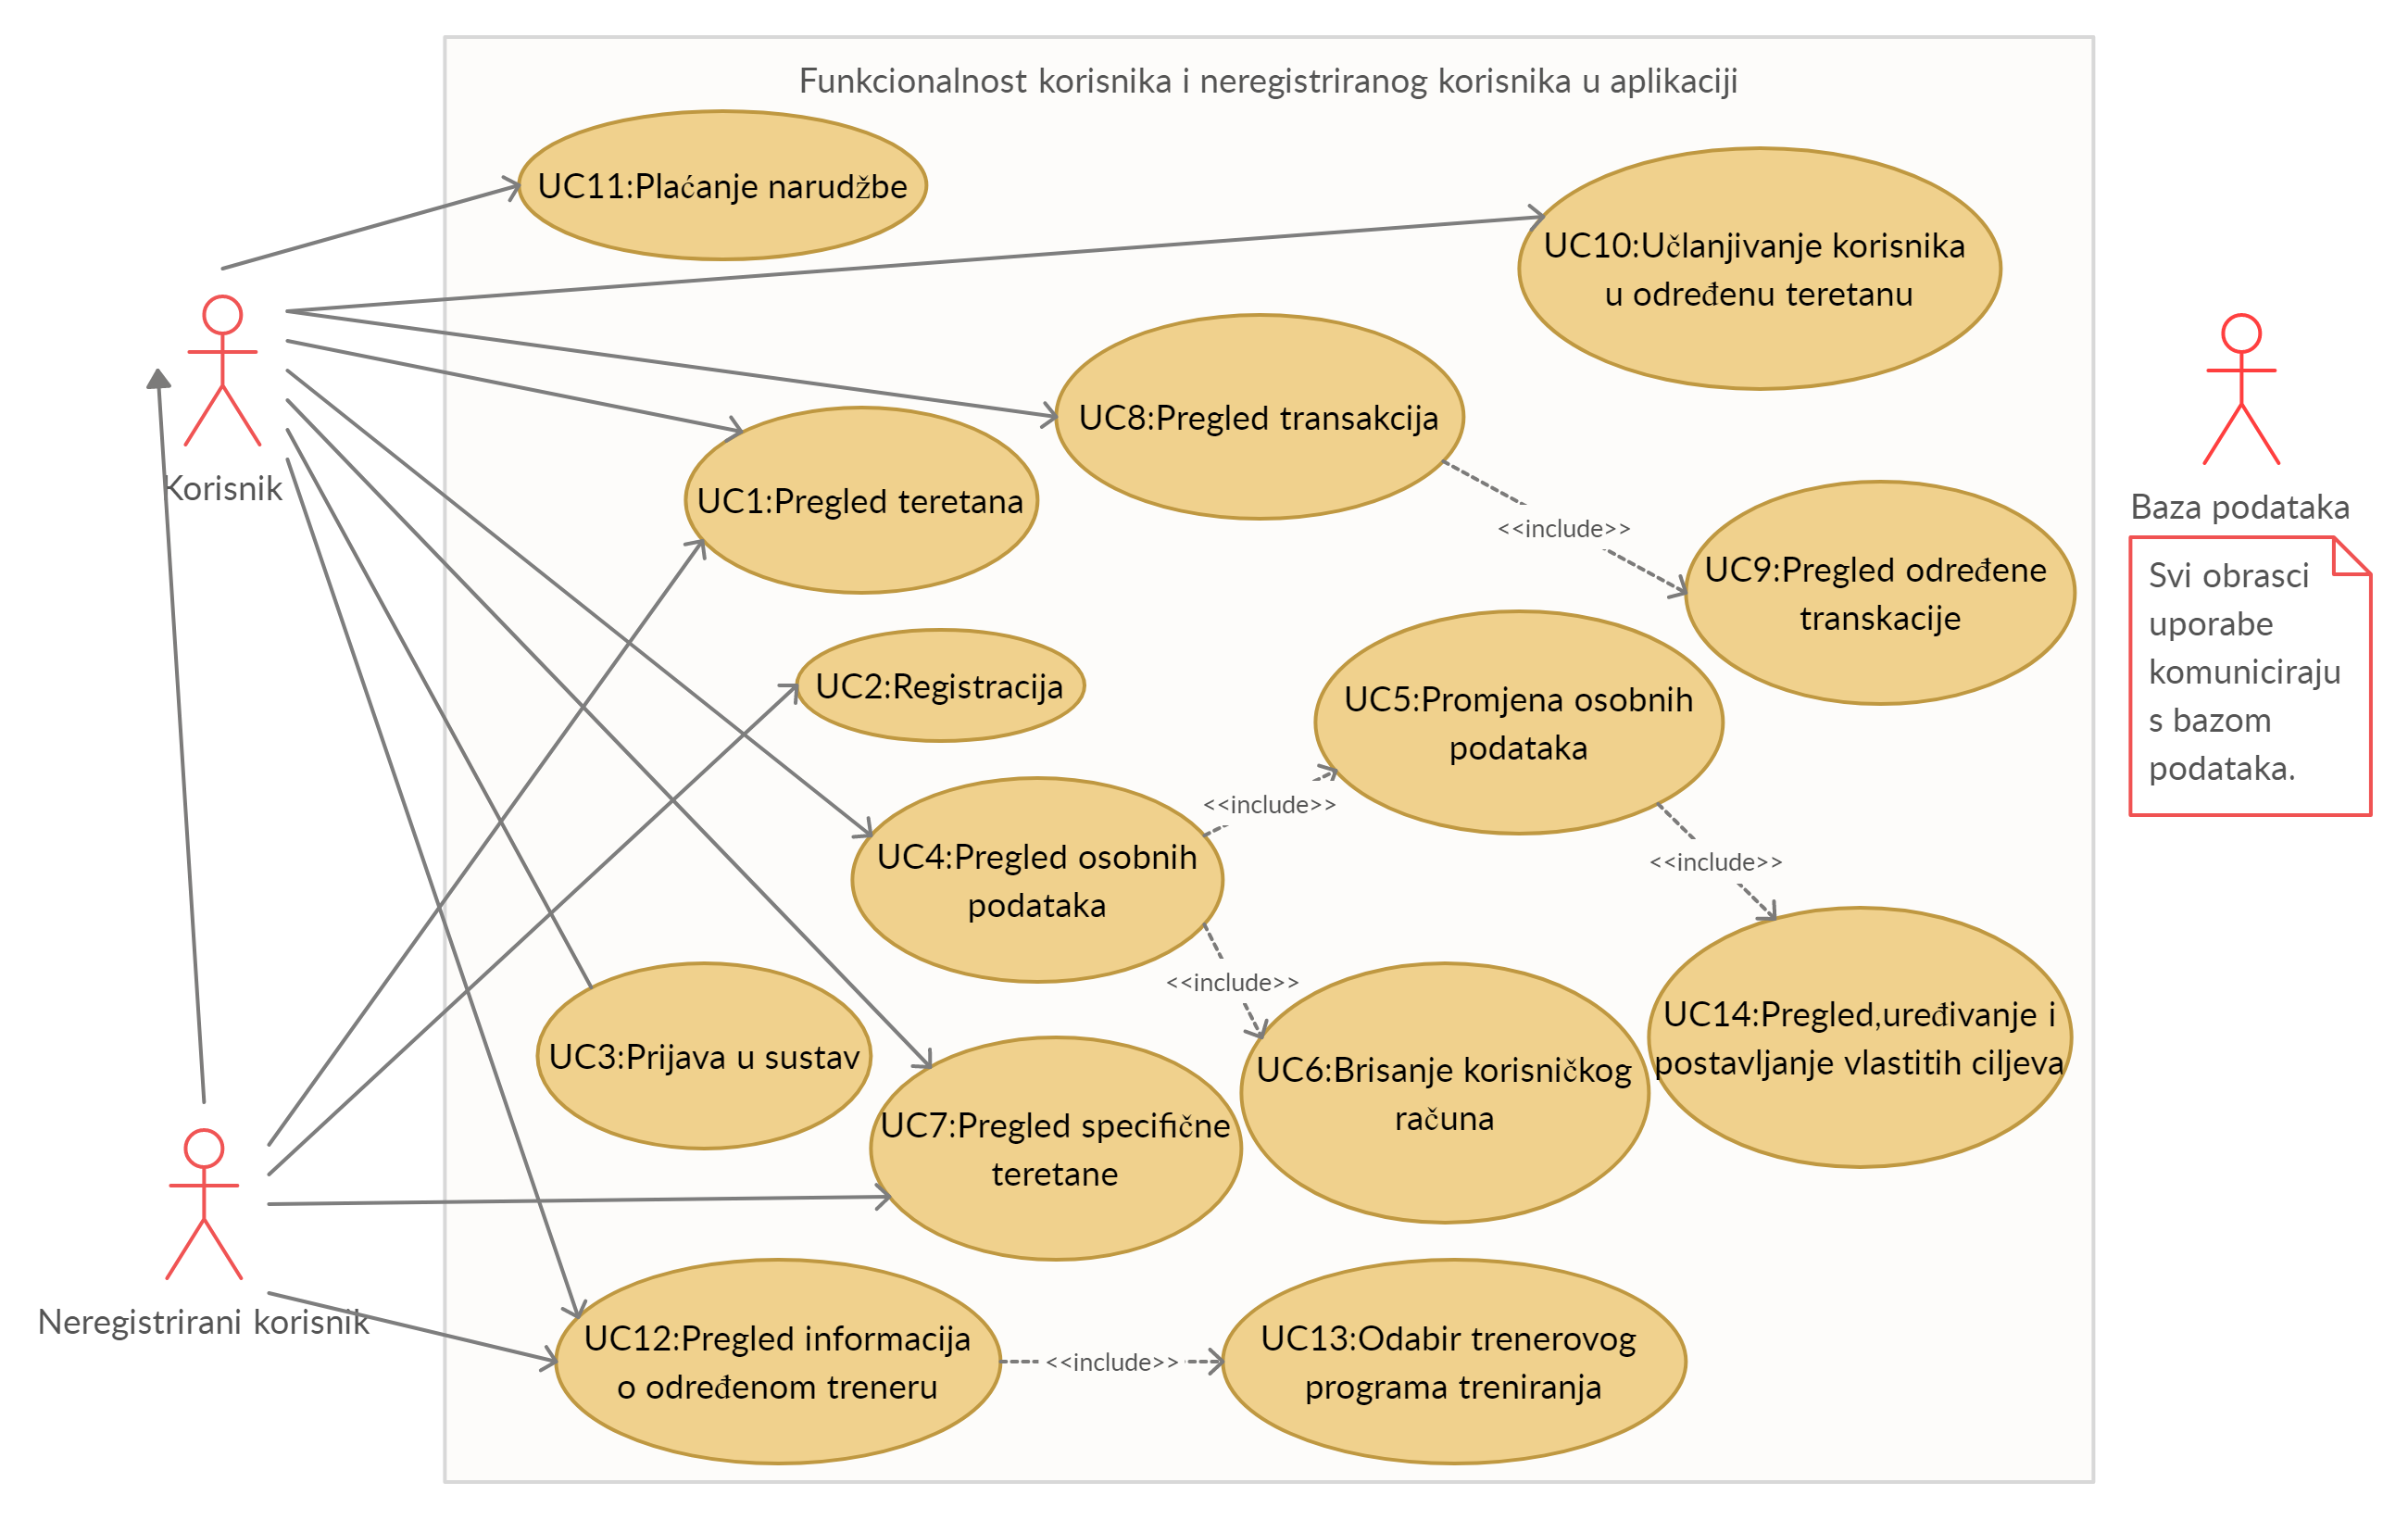
\includegraphics[height= 13cm,width=1.2\textwidth]{dokumentacija/slike/obrazac1.jpg}
				\textbf{Slika 3.1: Dijagram obrasca uporabe, funkcionalnost korisnika i neregistriranog korisnika u aplikaciji  }
				
				\end{figure}
				
				\begin{figure}
				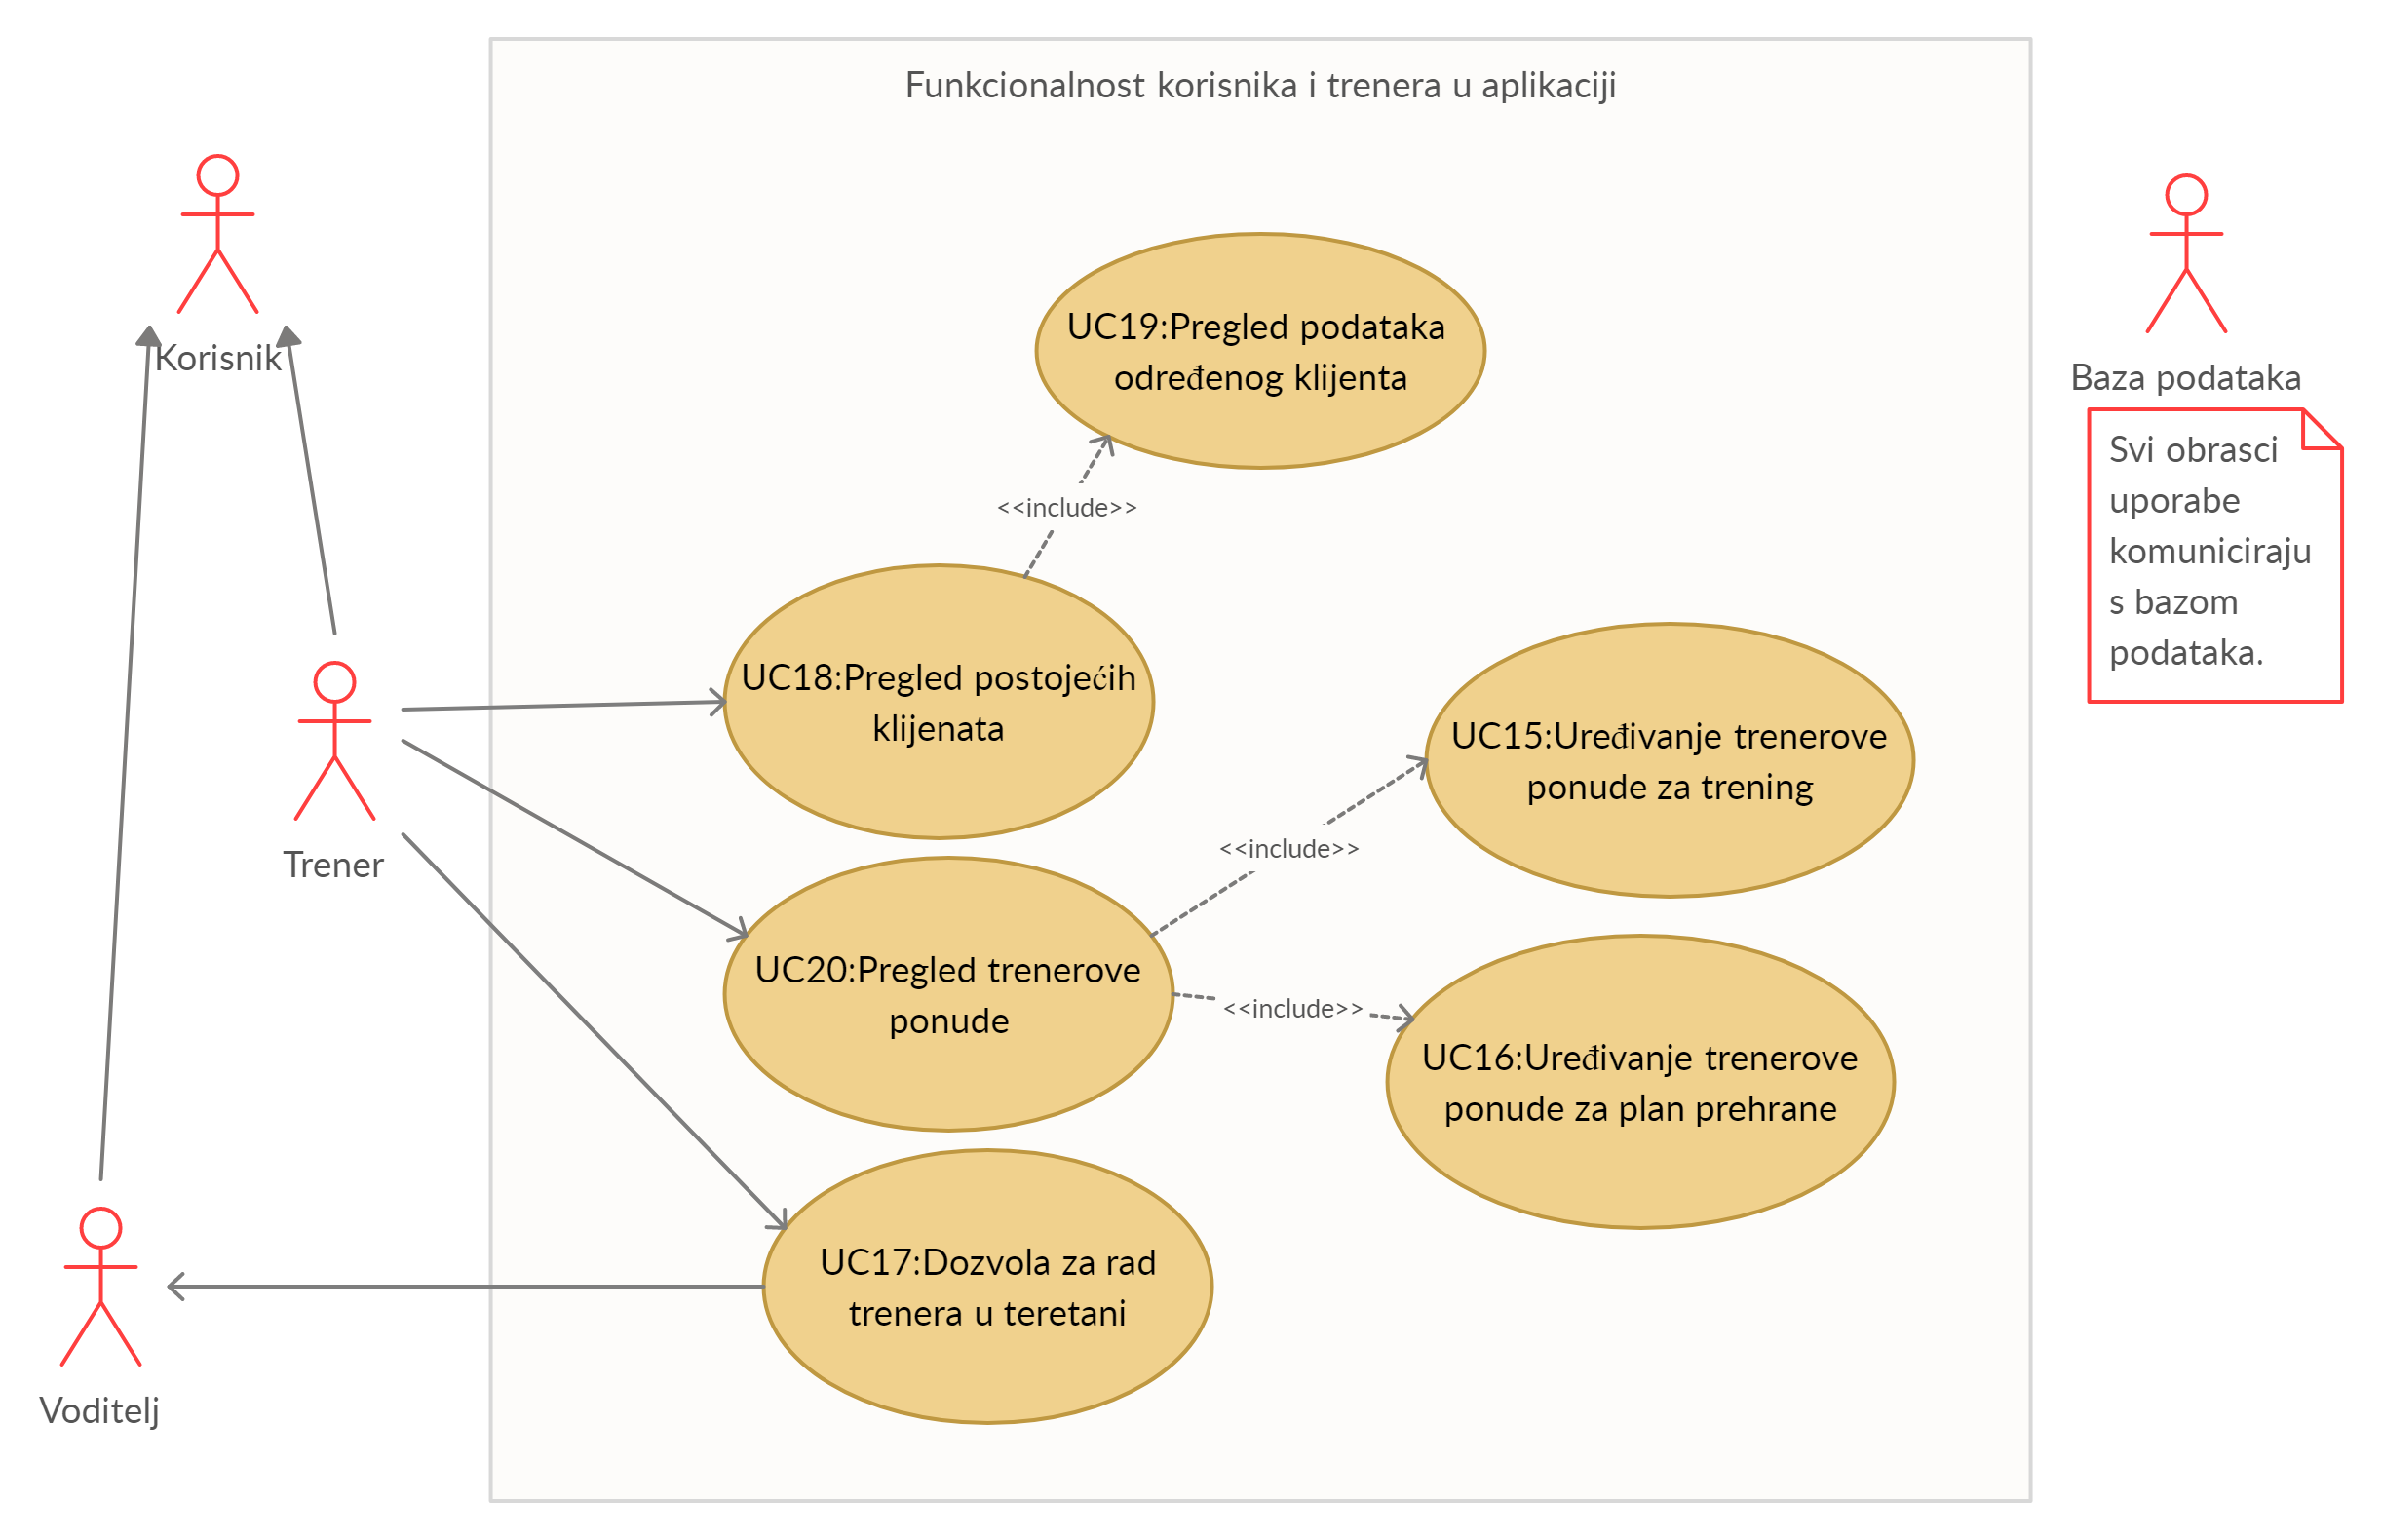
\includegraphics[height= 13cm,width=1.2\textwidth]{dokumentacija/slike/obrazac2.jpg}
				\textbf{Slika 3.2: Dijagram obrasca uporabe, funkcionalnost korisnika i trenera u aplikaciji}
				\end{figure}
				
				\begin{figure}
				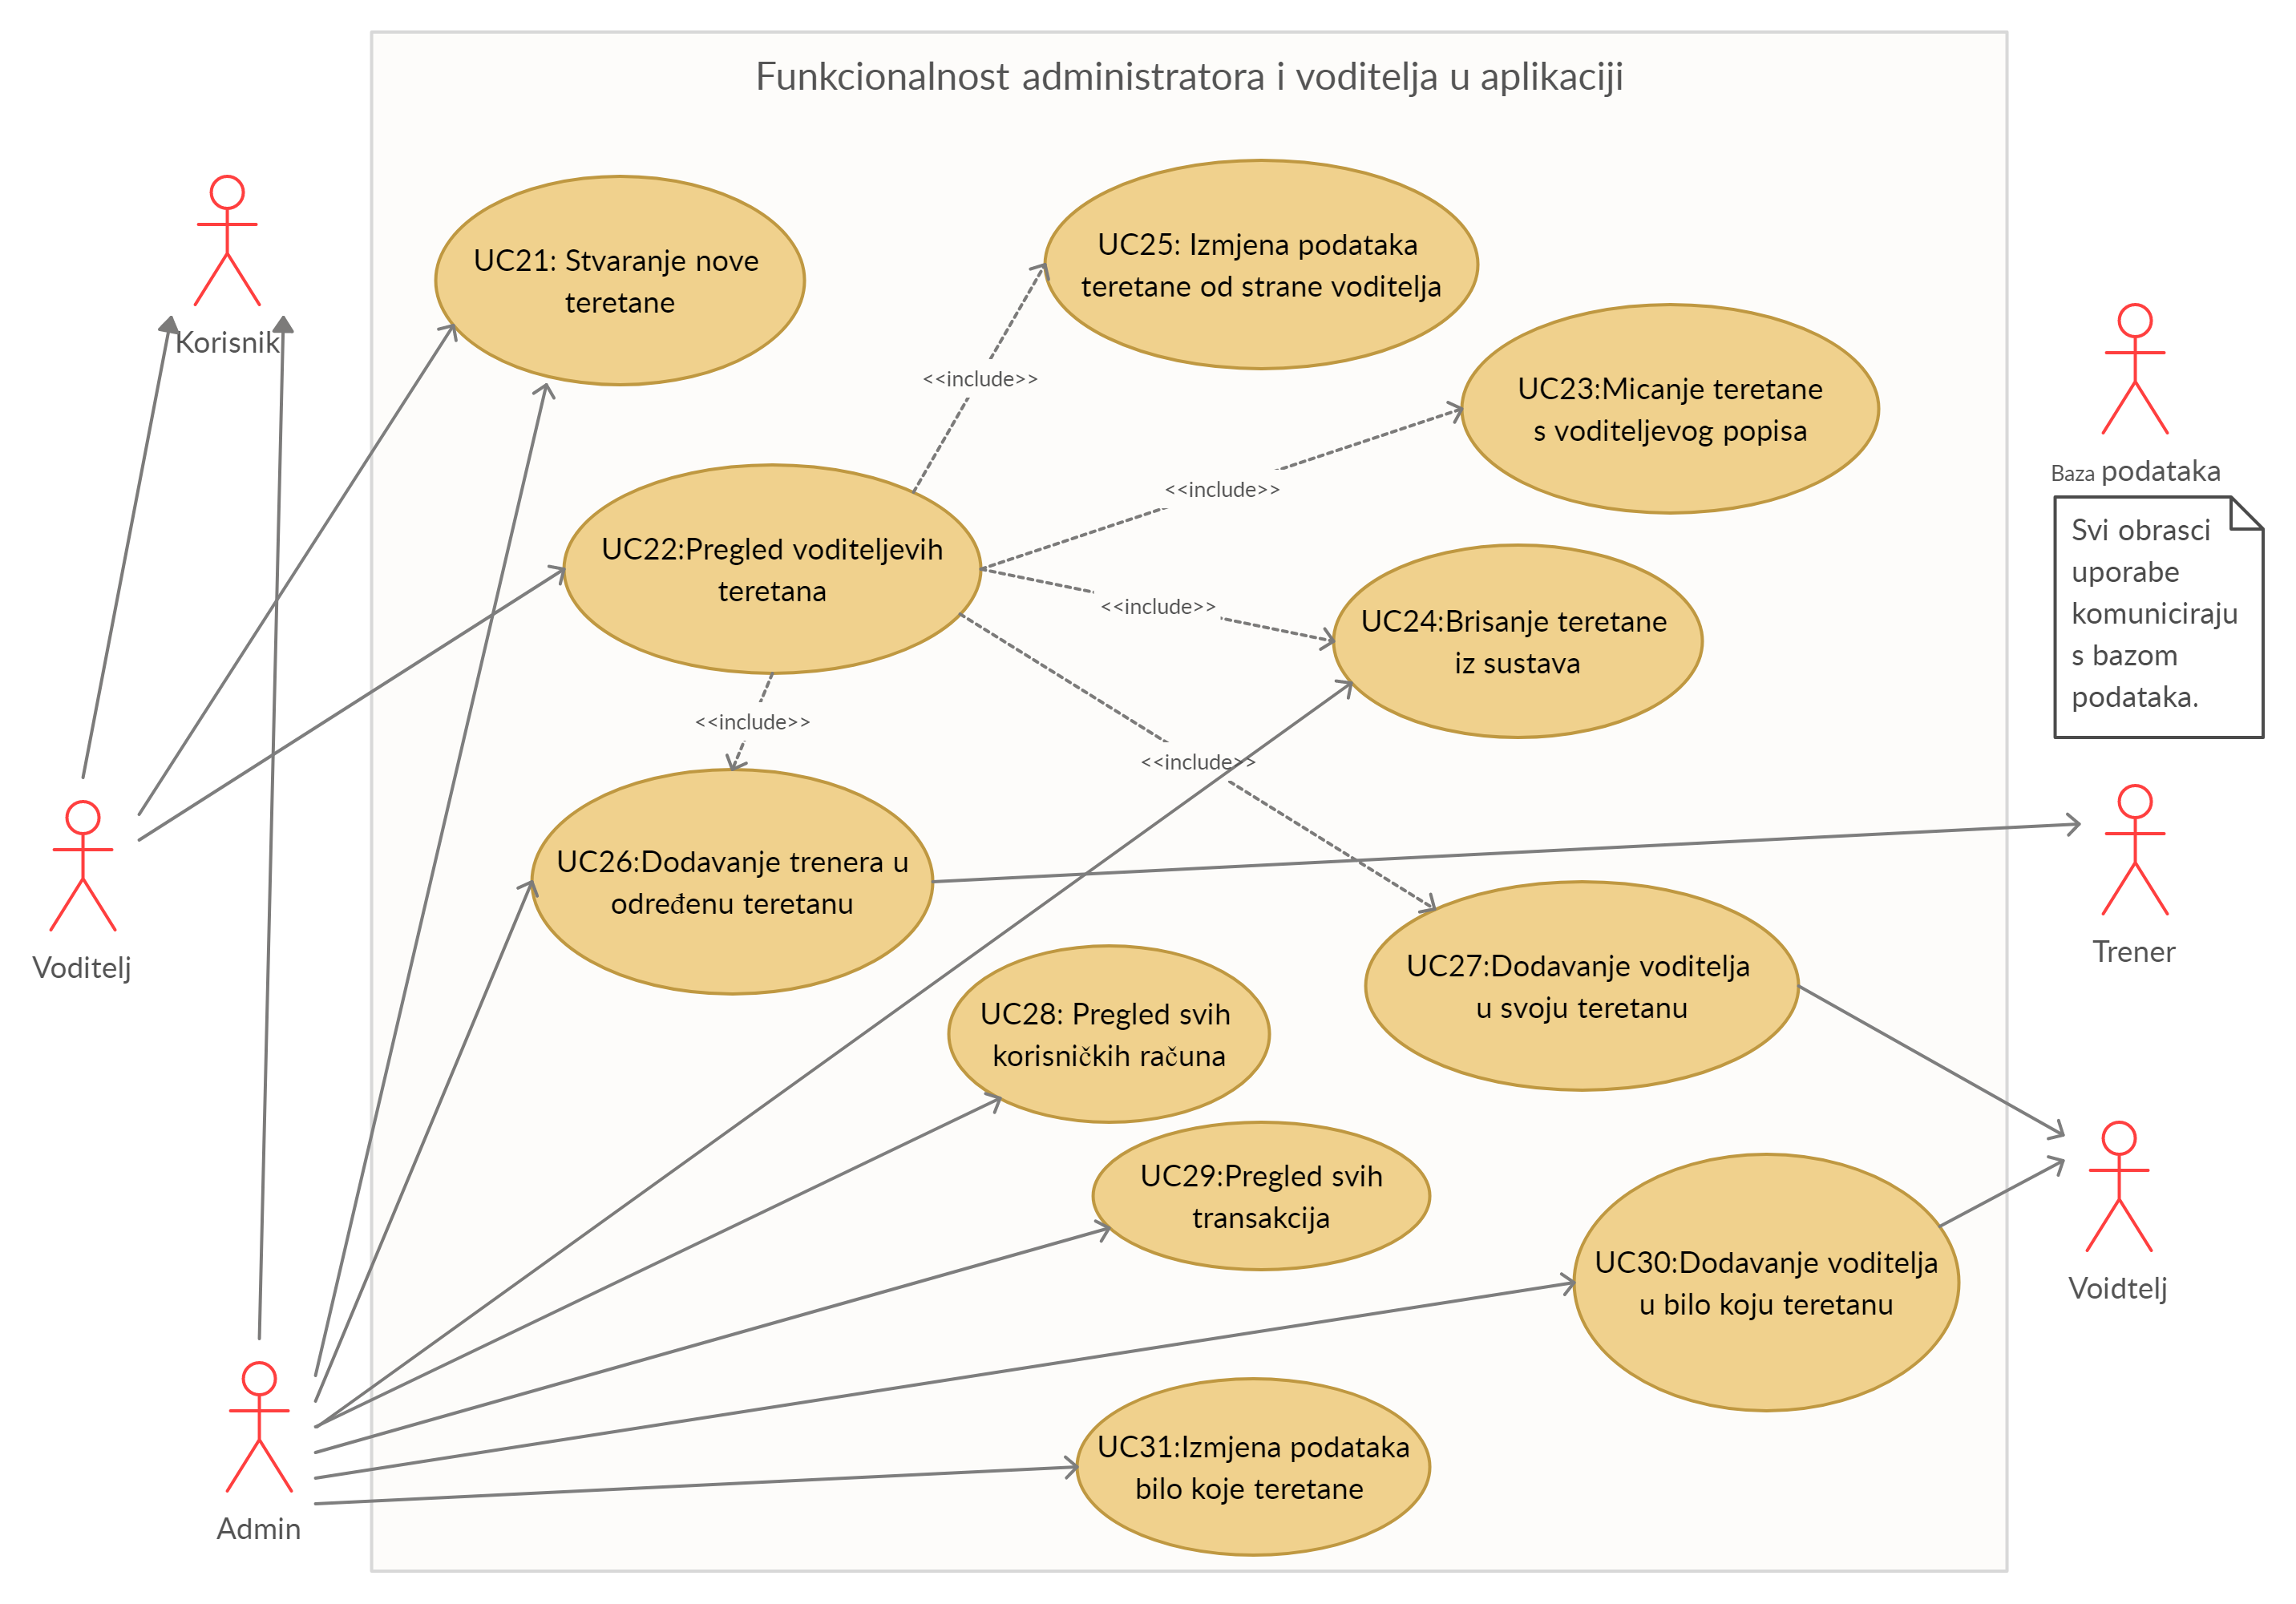
\includegraphics[height= 13cm,width=1.2\textwidth]{dokumentacija/slike/obrazac3.jpg}
				\textbf{Slika 3.3: Dijagram obrasca uporabe, Funkcionalnost korisnika i neregistriranog korisnika u aplikaciji}
				\end{figure}
				
					
				\eject	
				
		    
				
			\subsection{Sekvencijski dijagrami}
				
				\textbf{\textit{dio 1. revizije}}\\
				
				\textit{Nacrtati sekvencijske dijagrame koji modeliraju najvažnije dijelove sustava (max. 4 dijagrama). Ukoliko postoji nedoumica oko odabira, razjasniti s asistentom. Uz svaki dijagram napisati detaljni opis dijagrama.}
				\eject
	
		\section{Ostali zahtjevi}
		
			\textbf{\textit{dio 1. revizije}}\\
		 
			 \textit{Nefunkcionalni zahtjevi i zahtjevi domene primjene dopunjuju funkcionalne zahtjeve. Oni opisuju \textbf{kako se sustav treba ponašati} i koja \textbf{ograničenja} treba poštivati (performanse, korisničko iskustvo, pouzdanost, standardi kvalitete, sigurnost...). Primjeri takvih zahtjeva u Vašem projektu mogu biti: podržani jezici korisničkog sučelja, vrijeme odziva, najveći mogući podržani broj korisnika, podržane web/mobilne platforme, razina zaštite (protokoli komunikacije, kriptiranje...)... Svaki takav zahtjev potrebno je navesti u jednoj ili dvije rečenice.}
			 
			 
			 
=======
\chapter{Specifikacija programske potpore}
		
	\section{Funkcionalni zahtjevi}
			
			
			\noindent \textbf{Dionici:}
			
			\begin{packed_enum}
				
				\item Klijent teretane
				\begin{packed_enum}
					
					\item registrirani
					\item neregistrirani
					
				\end{packed_enum}
				\item Trener
				\item Voditelj teretane			
				\item Administrator
				\item Razvojni tim
				
			\end{packed_enum}
			
			\noindent \textbf{Aktori i njihovi funkcionalni zahtjevi:}
			
			
			\begin{packed_enum}
				\item  \underbar{Neregistrirani/neprijavljeni korisnik (inicijator) može:}
				
				\begin{packed_enum}
					
					\item pregledati popis svih teretana na platformi
					\item sortirati spomenuti popis prema sljedećim kriterijima: ime teretane, lokacija, trener
					\item otvoriti početnu stranicu svake teretane na kojoj se nalaze osnovne informacije (radno vrijeme, lokacija, cijena
					članarine…)
					\item izraditi administratorski, voditeljski, trenerski ili korisnički račun s namjerom treniranja u teretani za koje je potrebno navesti ime, prezime i email adresu, dok se može, ali ne mora dodati PayPal račun te je za izradu trenerskog korisničkog računa posebno potrebno navesti posebne podatke poput visine i težine
					
					
				\end{packed_enum}
			
				\item  \underbar{Klijent (inicijator) može:}
				
				\begin{packed_enum}
					
					\item pregledavati i sortirati popis registriranih teretana
					\item pregledavati i mijenjati osobne podatke
					\item izbrisati svoj korisnički račun
					\item plaćati članarine u teretanama putem interneta
					\item pregledavati sve izvršene transakcije u kojima su sudjelovali
					\item pregledavati popis teretana u kojima smiju vježbati, odnosno u kojima su platili članarinu
					\item kupovati planove prehrane i vježbanja od trenera
					\item ugovarati privatne ili grupne treninge
					\item voditi i pratiti napredak u vlastitom planu vježbanja
					
				\end{packed_enum}
			
				\item  \underbar{Trener (inicijator) može:}
				
				\begin{packed_enum}
					
					\item pregledavati i sortirati popis registriranih teretana
					\item pregledavati i mijenjati osobne podatke
					\item izbrisati svoj korisnički račun
					\item objavljivati ponude planova treninga i/ili vježbanja
					\item objavljivati i ugovarati termine privatnih i grupnih treninga u teretanama gdje imaju te ovlasti
					\item pregledavati sve izvršene transakcije u kojima su sudjelovali
					\item pregledavati popis teretana u kojima smiju djelovati, odnosno raditi (voditi treninge, planovi prehrane i sl.)
					\item nuditi usluge treniranja teretanama
					
				\end{packed_enum}
		
				\item  \underbar{Voditelj teretane (inicijator) može:}
				
				\begin{packed_enum}
					
					\item pregledavati i sortirati popis registriranih teretana
					\item pregledavati i mijenjati osobne podatke
					\item izbrisati svoj korisnički račun
					\item stvarati nove teretane u sustavu
					\item davati dozvolu drugim voditeljima da vode neke njegove teretane
					\item mijenjati važne informacije o teretanama (radno vrijeme, lokacija i sl.)
					\item dopuštati registriranim trenerima rad u teretanama koje vodi
					\item vidjeti sve izvršene transakcije na aplikaciji unutar vlastite teretane
					
				\end{packed_enum}
	
				\item  \underbar{Administrator (inicijator) može:}
				
				\begin{packed_enum}
					
					\item pregledavati i sortirati popis registriranih teretana
					\item pregledavati i mijenjati osobne podatke
					\item vidjeti sve korisničke račune
					\item izbrisati svoj korisnički račun
					\item stvarati nove i brisati postojeće teretane u sustavu
					\item pregledati sve izvršene transakcije u aplikaciji
					\item davati dozvolu  voditeljima da vode pojedine teretane
					\item mijenjati važne informacije o teretanama (radno vrijeme, lokacija i sl.)
					\item dopuštati registriranim trenerima rad u teretanama
					
				\end{packed_enum}


				\item  \underbar{Baza podataka (sudionik):}
				
				\begin{packed_enum}
					
					\item pohranjuje sve podatke o korisnicima
					\item čuva informacije o ulogama pojedinih korisnika
					\item pohranjuje podatke o svim teretanama, njihovim voditeljima, trenerima i članovima
					\item pohranjuje izvršene transakcije
					
				\end{packed_enum}
		
			\end{packed_enum}
			
			\eject 
			
			
				
			\subsection{Obrasci uporabe}
				
				\textbf{\textit{dio 1. revizije}}
				
				\subsubsection{Opis obrazaca uporabe}
					\textit{Funkcionalne zahtjeve razraditi u obliku obrazaca uporabe. Svaki obrazac je potrebno razraditi prema donjem predlošku. Ukoliko u nekom koraku može doći do odstupanja, potrebno je to odstupanje opisati i po mogućnosti ponuditi rješenje kojim bi se tijek obrasca vratio na osnovni tijek.}\\
					

					\noindent \underbar{\textbf{UC$<$broj obrasca$>$ -$<$ime obrasca$>$}}
					\begin{packed_item}
	
						\item \textbf{Glavni sudionik: }$<$sudionik$>$
						\item  \textbf{Cilj:} $<$cilj$>$
						\item  \textbf{Sudionici:} $<$sudionici$>$
						\item  \textbf{Preduvjet:} $<$preduvjet$>$
						\item  \textbf{Opis osnovnog tijeka:}
						
						\item[] \begin{packed_enum}
	
							\item $<$opis korak jedan$>$
							\item $<$opis korak dva$>$
							\item $<$opis korak tri$>$
							\item $<$opis korak četiri$>$
							\item $<$opis korak pet$>$
						\end{packed_enum}
						
						\item  \textbf{Opis mogućih odstupanja:}
						
						\item[] \begin{packed_item}
	
							\item[2.a] $<$opis mogućeg scenarija odstupanja u koraku 2$>$
							\item[] \begin{packed_enum}
								
								\item $<$opis rješenja mogućeg scenarija korak 1$>$
								\item $<$opis rješenja mogućeg scenarija korak 2$>$
								
							\end{packed_enum}
							\item[2.b] $<$opis mogućeg scenarija odstupanja u koraku 2$>$
							\item[3.a] $<$opis mogućeg scenarija odstupanja  u koraku 3$>$
							
						\end{packed_item}
					\end{packed_item}
				
					
				\subsubsection{Dijagrami obrazaca uporabe}
					
					\textit{Prikazati odnos aktora i obrazaca uporabe odgovarajućim UML dijagramom. Nije nužno nacrtati sve na jednom dijagramu. Modelirati po razinama apstrakcije i skupovima srodnih funkcionalnosti.}
				\eject		
				
			\subsection{Sekvencijski dijagrami}
				
				\textbf{\textit{dio 1. revizije}}\\
				
				\textit{Nacrtati sekvencijske dijagrame koji modeliraju najvažnije dijelove sustava (max. 4 dijagrama). Ukoliko postoji nedoumica oko odabira, razjasniti s asistentom. Uz svaki dijagram napisati detaljni opis dijagrama.}
				\eject
	
		\section{Ostali zahtjevi}
		
			\textbf{\textit{dio 1. revizije}}\\
		 
			 \textit{Nefunkcionalni zahtjevi i zahtjevi domene primjene dopunjuju funkcionalne zahtjeve. Oni opisuju \textbf{kako se sustav treba ponašati} i koja \textbf{ograničenja} treba poštivati (performanse, korisničko iskustvo, pouzdanost, standardi kvalitete, sigurnost...). Primjeri takvih zahtjeva u Vašem projektu mogu biti: podržani jezici korisničkog sučelja, vrijeme odziva, najveći mogući podržani broj korisnika, podržane web/mobilne platforme, razina zaštite (protokoli komunikacije, kriptiranje...)... Svaki takav zahtjev potrebno je navesti u jednoj ili dvije rečenice.}
			 
			 
			 
>>>>>>> devdoc
	